\documentclass[a2paper, portrait, 14pt]{tikzposter}
\usepackage[utf8]{inputenc}
\usepackage{amsmath}
\usepackage{amsfonts}
\usepackage{amssymb}
\usepackage{graphicx}
\usepackage{booktabs}
\usepackage{lmodern}
\renewcommand{\familydefault}{\sfdefault} % Use sans-serif for a modern look

% --- Modern & Minimalistic Styling ---
\usetheme{Simple}
\useblockstyle{Basic}
\usetitlestyle{Empty} % Minimalist title

% Define a professional color palette
\definecolor{Navy}{RGB}{0, 51, 102}
\definecolor{Snow}{RGB}{250, 250, 250}
\definecolor{Slate}{RGB}{70, 70, 70}

\colorlet{backgroundcolor}{white}
\colorlet{framecolor}{white}
\colorlet{titlefgcolor}{Navy}
\colorlet{titlebgcolor}{white}
\colorlet{blocktitlebgcolor}{Navy}
\colorlet{blocktitlefgcolor}{white}
\colorlet{blockbodybgcolor}{Snow}
\colorlet{blockbodyfgcolor}{Slate}
\colorlet{blockframecolor}{Navy}

% Metadata
\title{\parbox{\linewidth}{\centering \textbf{Uczenie silnika szachowego \\ na partiach o rosnącym Elo}}}
\author{
    Autor: Adam Zieliński \\
    Promotor: dr hab. Łukasz Mikulski, prof. UMK
}
\institute{Uniwersytet Mikołaja Kopernika Wydział Matematyki i Informatyki}
\date{\today}

\begin{document}

\maketitle

\block{}{
    \begin{center}
        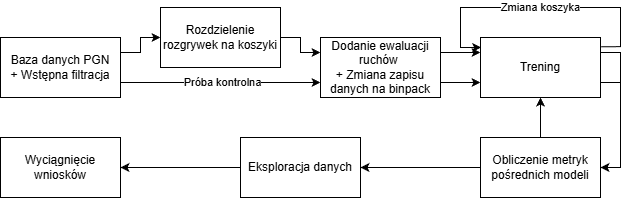
\includegraphics[width=0.5\linewidth]{workflow.png}
    \end{center}
}

\begin{columns}
    % --- COLUMN 1 ---
    \column{0.5}
    
    \block{1. Cel Badania}{
        \textbf{Badanie zachowania silnika NN podczas uczenia na danych o rosnącym poziomie umiejętności.}
        \begin{itemize}
            \item Analiza stosunku między Elo danych uczących a Elo powstałego modelu.
            \item Wpływ curriculum learning na prędkość nauki i styl gry.
            \item Porównanie modelu badawczego z modelem kontrolnym.
        \end{itemize}
    }

    \block{2. Hipotezy}{
        \begin{itemize}
            \item \textbf{H1: Szybsza nauka cech.} Model szybciej odnajdzie wzorce, gdyż gracze o niskim Elo kierują się mniej skomplikowanymi przemyśleniami niż arcymistrzowie.
            \item \textbf{H2: Ludzki styl gry.} Model na każdym etapie będzie grał podobnie do człowieka, unikając losowych ruchów charakterystycznych dla modeli uczonych na wszystkich taktykach naraz.
            \item \textbf{H3: Korelacja Elo.} Istnieje ścisła zależność między rankingiem zbioru treningowego a siłą gry modelu końcowego.
        \end{itemize}
    }

    \block{3. Metodologia}{
        \begin{itemize}
            \item \textbf{Start:} Wykorzystanie modelu znającego podstawy szachów w celu optymalizacji czasu obliczeń.
            \item \textbf{Dane:} Zbiory pogrupowane w koszyki Elo. Przejście do kolejnego koszyka po określonej liczbie epok lub osiągnięciu progu jakości.
            \item \textbf{Zapis:} Archiwizacja wag modelu po każdej zmianie przedziału i co określoną liczbę epok.
            \item \textbf{Kontrola:} Równoległy trening modelu na przemieszanym zbiorze danych (bez podziału na rangi).
        \end{itemize}
    }

    % --- COLUMN 2 ---
    \column{0.5}

    \block{4. Metryki}{
        \begin{itemize}
            \item \textbf{Elo:} Rozgrywane turnieje przeciwko silnikom ze znanym rankingiem.
            \item \textbf{Human-like Index:} Zgodność z ruchami ludzi.
            \item \textbf{Loss Curve:} Zmiana funkcji straty, szczególnie przy zmianie koszyka na lepsze Elo.
        \end{itemize}
    }

    \block{5. Spodziewane Wyniki}{
        \begin{center}
            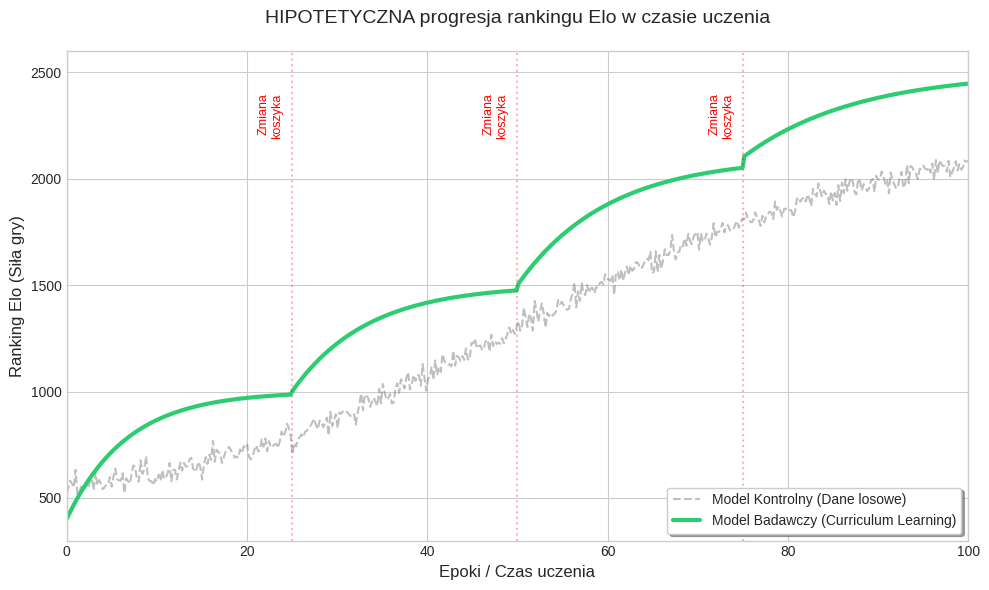
\includegraphics[width=0.9\linewidth]{hypothetical_plot.png}
        \end{center}
        Model badawczy szybciej odnajdzie cechy, wystąpią skoki rozwojowe
    }

    \block{6. Wnioski}{
        \begin{itemize}
            \item Weryfikacja akceleracji nauki przez prostsze dane.
            \item Ocena przewidywalności modelu dla człowieka.
            \item \textbf{Zastosowanie:} Asystent szachowy uczący się razem z użytkownikiem.
        \end{itemize}
    }
\end{columns}

\end{document}
